\documentclass{llncs}

\usepackage{hyperref}
\usepackage{graphicx}
\usepackage{epstopdf}
\usepackage{listings}
\usepackage{caption}
\usepackage[dvipsnames]{xcolor}
\usepackage{float}
\usepackage{geometry}\geometry{
a4paper,
left=10em,
right=10em
}

\newcommand\realnumberstyle[1]{}

\makeatletter
\newcommand{\zebra}[3]{%
    {\realnumberstyle{#3}}%
    \begingroup
    \ifodd\value{lstnumber}%
    \color{#1}%
    \else
    \color{#2}%
    \fi
    \ifnum\value{lstnumber} > 9
    \rlap{\hspace*{\lst@numbersep}\hspace*{0.6em}%
        \color@block{\linewidth}{\ht\strutbox}{\dp\strutbox}%
    }%
    \else
    \rlap{\hspace*{\lst@numbersep}\hspace*{0.23em}%
        \color@block{\linewidth}{\ht\strutbox}{\dp\strutbox}%
    }%
    \fi
    \endgroup
}
\makeatother

\makeatletter
\newcommand{\code}[1]{%
    \texttt{#1}%
    \fontdimen2\font=0.4em
    \fontdimen3\font=0.2em
    \fontdimen4\font=0.1em
    \fontdimen7\font=0.1em
    \hyphenchar\font=`\-
}
\makeatother

\lstset{
    mathescape,
    numbersep=10pt,
    breaklines=true,
    showstringspaces=false,
    breakatwhitespace=true,
    frame=b,
    framexleftmargin=15pt,
    framexbottommargin=5pt,
    framextopmargin=15pt,
    xleftmargin=\parindent,
    showstringspaces=false,
    basicstyle=\footnotesize\ttfamily,
    numberstyle=\zebra{gray!50}{gray!10}{}\tiny,
    keywordstyle=\color{red},
    commentstyle=\color{OliveGreen},
    captionpos=b,
}

\DeclareCaptionFormat{listing}{#1#2#3}
\captionsetup[lstlisting]{%
    format=listing,
    singlelinecheck=false,
    margin=0pt,
    labelfont=bf
}
\captionsetup[figure]{%
    format=listing,
    singlelinecheck=false,
    margin=0pt,
    labelfont=bf,
}

\begin{document}
\title{Time Synchronization II}

%If you're using runningheads you can add an abreviated title for the running head on odd pages using the following
%\titlerunning{abreviated title goes here}
%and an alternative title for the table of contents:
%\toctitle{table of contents title}

\subtitle{Rate-Based Synchronous Diffusion}

%For a single author
%\author{Author Name}

%For multiple authors:
\author{Pascal Gadient\\ Domenico Iapello \\ Felix Langenegger} 

%If using runnningheads you can abbreviate the author name on even pages:
%\authorrunning{abbreviated author name}
%and you can change the author name in the table of contents
%\tocauthor{enhanced author name}

%For a single institute
%\institute{Institute Name \email{email address}}

% If authors are from different institutes 
\institute{University of Bern \\ Communication and Distributed Systems\\AS2015}

%to remove your email just remove '\email{email address}'
% you can also remove the thanks footnote by removing '\thanks{Thank you to...}'

\maketitle

%\begin{abstract}
%abstract text goes here - Lorem ipsum dolor sit amet, consectetur adipiscing elit, sed do eiusmod tempor incididunt ut labore et dolore magna aliqua.
%\end{abstract}

\section{Protocol Introduction}
% Maximum 1 page about the theoretical basics of the experiment.
A sensor network is basically made of some sensor nodes that are linked together. To fulfil the main goals of the sensor network the time synchronisation of the network nodes is important.  For example, it is useful to have the same time frames on each node to compare the measurements of each node. Or if the network is a mobile sensor network, the exact localisation of each node could be demanded, which can only be provided, if the nodes have a synchronised time. Additionally, the coordination of duty cycles can only be performed if the nodes are in synchronisation.\\
\indent The requirements of an accurate time synchronisation algorithm are amongst others, precision, energy efficiency, a small memory footprint, scalability and robustness. Most of all, the time synchronisation is not the main application of the node itself, so the algorithm should not consume most of the energy and processing resources for this task. The same goes for the memory. The time synchronisation algorithm should be scalable in two dimensions. Firstly, it has to be scalable to many different resource-constrained devices, that means it should run on nodes with very small resources as well as on devices with high-end circuitry. Secondly, it should be scalable from small to large sensor networks. In other words, the algorithm should run as robust as possible independently of the number of nodes.\\
\indent This project report explains how we solved the problem of time synchronisation based on the Rate-Based Synchronous Diffusion Algorithm (RBSDA)\footnote{See lecture slide: V. Time Synchronization - 3.3.1 Diffusion-based Synchronization p. 29-30. This slides are based on the paper: Global Clock Synchronization in Sensor Networks by Qun Li and  Daniela Rus\cite{LiRus2006}}. The basic idea of the RBSDA is to know all the visible nodes of one specific node, and then to iterate over the known neighbours to determine the time offset via round-trip synchronisation.\\

\section{Methods}
%Especially, describe the methods used to realize the protocol (functions in the code and their functionality)

First, we will speak in detail about the synchronisation algorithm itself and discuss how it works. Later, we pinpoint some programming specialities of the used sensor nodes and finally, we present some debugging habits and methods used to ensure a fully functional implementation.\\
\indent The synchronisation algorithm progresses in three steps: Initially, the sensor node generates an internal representation of the surrounding neighbour nodes. Afterwards, it sends round-trip-time (RTT) request packets to all discovered nodes and stores then the received RTT of each node together with the remote timestamp into the previously created neighbours node table representation. Finally, we calculate the median of all skews with respect to the RTTs and adjust therefore the local node time with these results multiplied by a constant factor alpha. We repeat the steps starting with the RTT request as long as we try to stay in synchronisation with the other nodes (in general this is equivalent to the lifetime of a node).
However, we consider only half the RTT, because the time set by the remote node travels only from the remote node to the corresponding node, i.e. half of the RTT time is used. The fundamental principle of this process is described in pseudo-code at listing \ref{lst:algo}.

\begin{lstlisting}%
[language=C, numbers=left, caption={Diffusion algorithm (DA) used to synchronise the whole sensor network.}, label={lst:algo}]
//Do the following with some given frequency
for each sensor $n_i$ in the network do
  Exchange clock times with $n_i$'s neighbours
    for each neighbour $n_j$ do
      Let the time difference between $n_i$ and $n_j$ be $(t_i - t_j)$
        Change $n_i$'s time to $t_i - r_{ij} (t_i - t_j)$
\end{lstlisting}
\noindent On a high-level perspective this converges, because each node adjusts itself towards the time of its neighbours. Hence, the more neighbours are seeing each other, the faster will the synchronisation take place. However, if there are some partition-like structures in the network it will still converge, but we will encounter disproportional long synchronisation sequences. This is the result of a few nodes that form a bridge between two different time clusters, so all time adjustments between both clusters will involve these few nodes. Thus, the impact on the whole network is proportionally small, caused by the median calculations (a big skew divided by the amount of (many) nodes results in a small correction value). Last, but not least, the alpha value only guarantees a convergence while being roughly in the range [1, 10]. Hence, with an alpha value of ten, the average synchronisation accuracy would be at most ten clock ticks, further it would take significantly more time to converge than with smaller values (as explained in detail in section four).\\
\indent In the listing below \ref{lst:code} we can easily see several specialities that occur in general on embedded devices such as our used sensors: i) Floating-point unit does not exist, hence, we have to use integer divisions instead of floating-point multiplications as in line seven. ii) Most hardware-specific system calls are not that well documented, we assume this is an outcome of embedded CPU designers, that set the focus on the chip, rather than the diverse operating systems that drive the chip, shown in line 17. iii) C code is used in general, as a result of the small memory and CPU footprint requirement.
\begin{lstlisting}%
[language=C, numbers=left, caption={RBSDA-Algorithm --- Skew Adjustment},label={lst:code}]
static void updateMyTime() {
  totalClockSkew = 0;
  activeNeighbourCount = 0;
  for (i5 = 0; i5 < MAX_NEIGHBOURS; i5++) {
    if (neighbours[i5].activeState) {
      activeNeighbourCount += 1;
      totalClockSkew += neighbours[i5].skew / ALPHA;
      neighbours[i5].skew = 0;
      neighbours[i5].rtt = 0;
      neighbours[i5].activeState = 0;
    }
  }
  if (activeNeighbourCount > 0) {
    totalClockSkew = totalClockSkew / activeNeighbourCount;
    clockCorrection = clock_time() + totalClockSkew;
    clock_set(clockCorrection, clockCorrection);
  }
}
\end{lstlisting}
\noindent While contributing to this project, we were in need of many different debugging strategies, because C programming can be very painful, especially for team members that are not so experienced with low-level programming. So we developed strategies that can be roughly assigned into one of these two classes: Syntax-Supporting Strategies (SSS), as well as Logic-Supporting Strategies (LSS). A prime example of the SSS is the separately maintained ``Playground.c" file in which we performed sandbox runs of some complicated code blocks, that upon successful validation eventually got in the main code base.\\
\indent In contrast the LSS consist of mainly three approaches: i) Simplification of the code as much as possible (i.e. using structs for message exchanges and internal data representations and trying to reduce code complexity in general). ii) Analysis and verification of the generated logs. iii) Creation of decision-trees for sophisticated code blocks.\bigbreak
\noindent For better comprehension we expose some basic routines that ensure a fully functional implementation. Booting up a node results in loading two network protocol stacks, technically speaking, the unicast and the broadcast message handlers. Whilst the broadcast module disseminates the node id along the neighbour nodes within the main program loop, the broadcast receiver block \code{recv\_bc(...)} recognises these messages and stores the corresponding neighbours in the node neighbours table with \code{addNeighbour(unsigned short id)}. Further in the main loop the code requests RTTs via unicast messages from all neighbours stored in the neighbours table with \code{requestRTT(unsigned short id)}. As soon as they get replied, the \code{recv\_uc(...)} callback method extends the table with the received data via \code{saveRTT(unsigned short id, unsigned short rtt, signed long skew)}.\\
After polling each neighbour, the own time gets adjusted by \code{updateMyTime()}. Accordingly, the saved RTT and skew data gets deleted and the process repeats again the main program loop.\\
\indent Some more casual methods can be found in the code as well. For example, there exist some led enabler and disabler methods with the corresponding callbacks (\code{enableLED(int color), disableLED(int color)}), as well as print methods for additional debugging like \code{print\-Neighbor\-List()}, or the \code{calcTimeDifference(unsigned short actualTime\-Own, unsigned short rttCorrTimeOther)} method used to calculate the time difference based on the time of two nodes with respect to clock overflows.
%\newpage
\section{Experimental Setup \& Measurement Procedure}
For the lecture `Sensor Network and Internet of Things' each group got two sensor nodes called `TelosB' which were assembled by Crossbow\footnote{The datasheet for the node is available on \url{http://www.willow.co.uk/TelosB_Datasheet.pdf}}. The node runs an operating system called Contiki\footnote{Contiki is a popular internet of things operating system, \url{http://www.contiki-os.org/}}. The assignment for the project was divided into two iterations. The first phase was about to implement a prototype of the algorithm, which we planned to run on four nodes. In the second phase we had to adapt the software, so that it can run on the TARWIS\footnote{TARWIS is a UI framework for wisebed solutions, \url{http://www.wisebed.eu/\#testbeds_ubern}} network with up to 40 nodes.\\
\indent In the beginning we inspected carefully each print statement in the console, but as further we came, the less feasible it got. Hence, we began to write parsers for different purposes which can, in combination with some plotting scripts, nicely visualise the outcome of the synchronisation process.

\section{Results and Analysis}
In this section we present some gathered results from our experiments, as well as some additional explanations and interpretations. The experiments consist of as less as four nodes in local execution and scale between 10 up to 40 nodes for the testbed runs. We run the experiment locally and on TARWIS with these three different configurations:\\ i) Normal run, ii) Fast run, iii) Fast run with some node resets after 55 minutes.\\
We performed additional measurements with different alpha values apart from the previously mentioned three setups.\\
\indent Important side mark for TARWIS results: It lies in the nature of a heavily used and commonly shared testbed at a remote location that the results are not every time perfectly deterministic. This may be caused by accidentally performed system maintenance on-site, other users that are requesting much capacity at that time, or workload that uses some shared resources on the specific cluster. Therefore, we had to use larger timeouts and intervals on TARWIS as with the local setup to obtain valid results.
\begin{figure}[H]
\centering
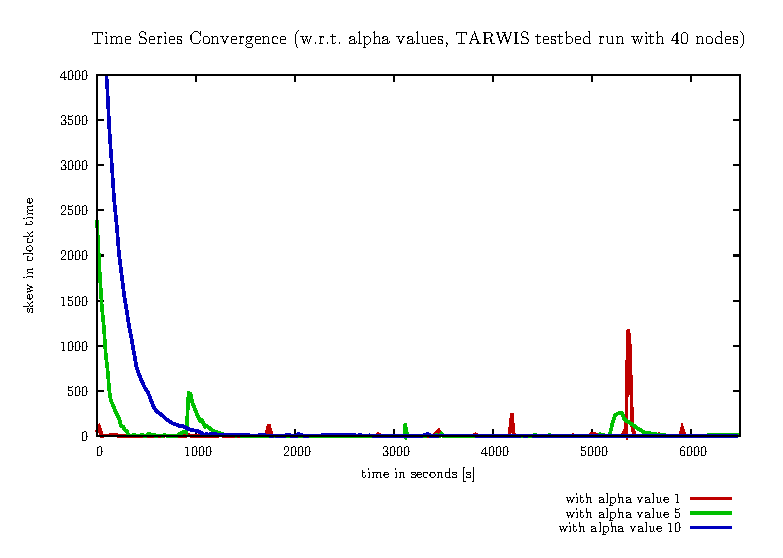
\includegraphics[scale=0.6]{images/FIG_01.eps}
\caption{Time series convergence with respect to alpha values}
\label{fig:alpha}
\end{figure}
\noindent In figure \ref{fig:alpha} we can clearly see that the algorithm is able to reach convergence around 250 seconds with a default alpha value of five. The small amplitudes in the figure are non-deterministic interferences within the sensor network. When we now enlarge the alpha value by a factor of two, the algorithm performs worse, because then the differences are only taken into account at small steps. Hence, the convergence phase takes more than twice as long including some random update interval waits. Very important to notice is that the sensitivity to external interferences decreases with incresing alpha values.\\
\begin{figure}[H]
\centering
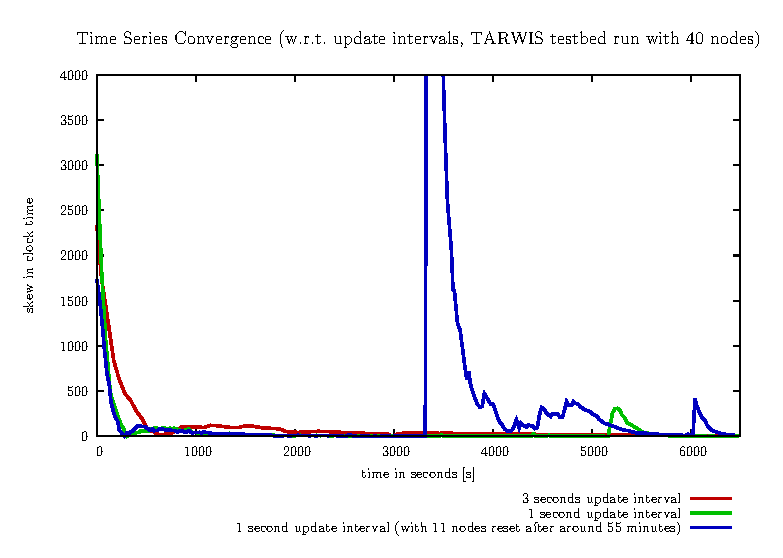
\includegraphics[scale=0.6]{images/FIG_02.eps}
\caption{Time series convergence with respect to update intervals}
\label{fig:update_intervals}
\end{figure}
\noindent On the other hand when we decrease the time synchronisation update interval, we can see that the assimilation of the nodes responds in an almost linear way to these changes, i.e. when we set the interval three times as high, the assimilation phase lasts roughly for three times the duration as well. We visualise this in figure \ref{fig:update_intervals}. In addition, a spike can be identified where some nodes have been reset.\\

\begin{figure}[H]
\centering
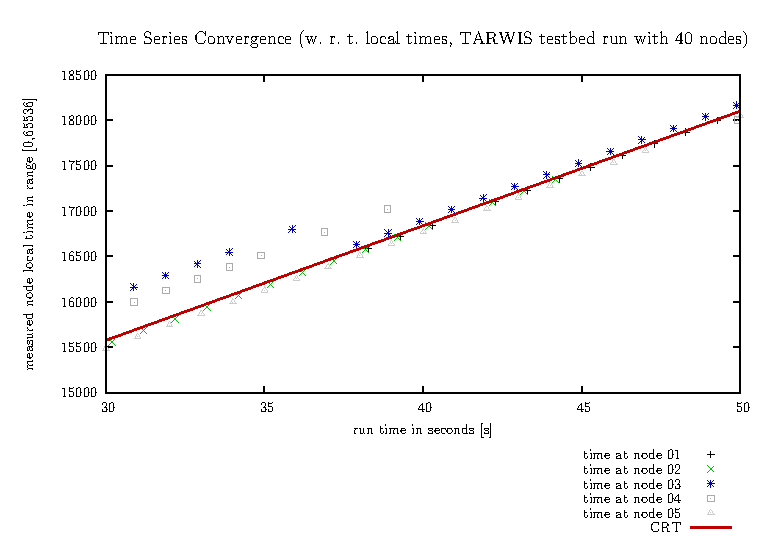
\includegraphics[scale=0.6]{images/FIG_03.eps}
\caption{Time series convergence with respect to some node's local time}
\label{fig:local_time}
\end{figure}

\noindent Next, we analyse the clock value over time. In figure \ref{fig:local_time} we see vertically each nodes current clock value at a specific point in time (x-axis). The gaps are representing the random waits of the node, before it starts the next RTT request cycle. The random waits is a result of introducing some randomness, because we want a guarantee that the nodes would not interfere each other in a repetitive way. We see that all lines are slowly pointing towards a common center line, we call this the cluster reference time (CRT). This CRT can be determined for each single node with respect to the neighbours and it is  increasing in any plot per definition. In the end it is our goal to ensure as accurate as possible that the CRT is the same for all nodes. Please consider, that the plots only visualise a small fraction of the synchronisation process inside a specific node (hence, it represents even a smaller field in the whole sensor network).\\
\indent Nevertheless, we were also interested in the discovery time of the neighbours. We saw in our experiments, that  in most cases all neighbours could be identified after 60 seconds. In some specific cases, this interval was much larger for some nodes. These nodes appear to have encountered a crowded channel, or poor signal strength in general.\\
\indent For all runs we obtained a maximal accuracy around the value of alpha. This can easily be explained: The changes being made to each nodes clock are \code{(calculated\_mean\_skew / alpha)} and the device doesn't contain a float\-ing-point unit (FPU), so as an example, all averaged skews smaller than five for an alpha set to five result in a skew change of zero. Anyhow, in our experiments occur still some values below this boundary, these anomalies are mainly caused by the nature of the dynamic system itself, when nodes independently of each other assimiliate themselves.

\section{Conclusions}

We were able to implement the demanded work and the results were quite promising. We reached an accuracy of converged networks that laid within the mathematical boundaries provided by the given skew update formula. Nevertheless, we found that the accuracy and the convergence speed depend highly on the used parameters. We identified an alpha value around five to be the most robust solution with respect to convergence speed, whereas the update interval should be defined as small as possible to ensure a quick assimilation. If the interval was set too low, the TARWIS testbed crashed and was not able to respond anymore. In our experiments we found an update interval of one second to be the best trade-off between reliability and convergence speed. In retrospect, it was a very reasonable decision to start with only two nodes and incrementally add one after another. This way we were able to identify and eliminate most bugs before they could appear in complex environments such as TARWIS, in which debugging is actually difficult. Network outages or spurious disconnects did not disrupt our solution, because in the worst case scenario this only would lead to new time skews within the network, that again can be reduced by our developed solution.\\
\indent Whatsoever, there are still some open issues that must be discussed further and should be considered beforehand our solution gets used in a production environment. The non-conclusive list of issues notably contains: i) Malicious nodes that inject random skews, ii) Ongoing large outages of the network in a way, the network is never able to reach a converged state, or iii) Varying algorithm processing speed on different hardware platforms in a heterogenous network.

\bibliography{biblio}{}

%The bibliography, done here without a bib file
%This is the old BibTeX style for use with llncs.cls
\bibliographystyle{splncs}

%Alternative bibliography styles:
%the following does the same as above except with alphabetic sorting
%\bibliographystyle{splncs_srt}
%the following is the current LNCS BibTex with alphabetic sorting
%\bibliographystyle{splncs03}
%If you want to use a different BibTex style include [oribibl] in the document class line


\end{document}

